\documentclass[12pt]{aghdpl}
\newcommand{\dotnet}{.NET}
\newcommand{\docker}{Docker}
\newcommand{\https}{HTTPS}
% Use and configure packages
\usepackage{graphicx}
\graphicspath{{./Assets/}}

\usepackage{float}
% \documentclass[language=en,11pt]{aghdpl}  % praca w języku angielskim

%---------------------------------------------------------------------------

\author{Bartłomiej Kręgielewski}
\shortauthor{B. Kręgielewski}

\titlePL{Aplikacja webowa do kolejkowania, uruchamiania i analizy symulacji}
\titleEN{Web app for queueing, running and analyzing simulations}

\shorttitlePL{Aplikacja webowa do kolejkowania, uruchamiania i analizy symulacji} % skrócona wersja tytułu jeśli jest bardzo długi
\shorttitleEN{Web app for queueing, running and analyzing simulations}


% Dopuszczalne wartości[1,2]:
% * "Projekt dyplomowy" - na koniec studiów I stopnia
% * "Praca dyplomowa" - na koniec studiów II stopnia
% [1] Zasady dyplomowania w roku akademickim 2020/2021 (Decyzja Dziekana WEAIiIB nr 16/2020 z dnia 9 grudnia 2020 roku)
% [2] Załącznik nr 1a) do Decyzji nr 16/2020 Dziekana Wydziału EAIiIB z dnia 09 grudnia 2020 r.
\thesistype{Praca dyplomowa}
%\thesistype{Master of Science Thesis}

\supervisor{dr hab. inż. Jarosław Wąs, prof. AGH}
%\supervisor{Jarosław Wąs, PhD}

\degreeprogramme{Informatyka}
%\degreeprogramme{Computer Science}

\date{2022}

%\department{Katedra Informatyki Stosowanej}
%\department{Department of Applied Computer Science}

\faculty{Wydział Elektrotechniki, Automatyki, Informatyki i Inżynierii Biomedycznej}
%\faculty{Faculty of Electrical Engineering, Automatics, Computer Science and Biomedical Engineering}

\acknowledgements{Serdecznie dziękuję dr. hab. inż. Jarosławowi Wąsowi, prof. AGH za objęcie mojej pracy dyplomowej swoją opieką oraz wsparcie w procesie jej tworzenia. Dziękuję również moim rodzicom i rodzeństwu za nieustanne wsparcie oraz koleżankom i kolegom z studiów, za ich opinie i rady.}

\begin{document}

\titlepages
\RedefinePlainStyle

\setcounter{tocdepth}{2}
\tableofcontents
\clearpage

\chapter{Wstęp}
\label{cha:wstep}
% TODO Add some bibliography regarding Moore's Law
\par Symulacje komputerowe służą nam do rozmaitych celów. Od prostych symulacji mających na celu przedstawienie działania jakiegoś zjawiska do naprawdę zaawansowanych, wieloagentowych systemów, mających na celu przewidzenie zachowania tłumu podczas opuszczania obiektu sportowego po wieczornym meczu siatkówki. Informacje uzyskiwane w ten sposób pomagają inżynierom na całym świecie projektować lepsze systemy, znajdować niedopatrzenia w już istniejących, jak i je optymalizować. Jednak aby osiągnąć te cele potrzebna jest znacząca moc obliczeniowa, którą często nie dysponujemy, używając komputerów osobistych. Nawet jeżeli szybkość z jaką urządzenia, które znajdują się pod lub na naszych biurkach, potrafią dokonywać obliczeń rosła przez ostatnie dziesięciolecia zgodnie z Prawem Moore'a, to tak samo rosły nasze oczekiwania wobec nich. Kiedy dziś mówimy o optymalizacji procesów, symulowaniu zjawiska fizycznego czy wspomnianej wcześniej symulacji środowiska składającego się z wielu agentów, to chcemy przeprowadzić nie jeden czy dwa eksperymenty, ale setki lub nawet tysiące.

\par Problem ten pozwala nam rozwiązać tak zwany \emph{Cloud Computing}. Oferuje on możliwość oddelegowania obliczeń do specjalnie przeznaczonego serwera (bądź też serwerów). Takie rozwiązania istnieją już w sieci, jednak jeżeli zaczniemy się im przyglądać, to dostrzeżemy, że większość z nich skłania się ku symulacjom konkretnych zjawisk fizycznych po dostarczeniu pliku w odpowiednim formacie. Jest to dość istotne ograniczenie, szczególnie kiedy interesują nas symulacje innej natury. Oczywiście trzeba wspomnieć również o superkomputerach, których reprezentantem jest między innymi znajdujący się w Cyfronecie AGH \emph{\prometheusAgh{}}. Maszyny te są jednak trudno dostępne. Uruchomienie na nich jakikolwiek obliczeń wymaga zazwyczaj otrzymania specjalnej zgody (grantu w przypadku \emph{\prometheusAgh{}}a), jak i samodzielnego przygotowania pewnego rodzaju systemu, który uruchamiałby automatycznie przygotowaną przez na symulację.

\par W mojej pracy inżynierskiej poruszam przedstawione powyżej problemy oraz proponuję ich rozwiązanie.

%---------------------------------------------------------------------------

\section{Zakres pracy}
\label{sec:zakresPracy}

Zakresem pracy jest:
\begin{itemize}
	\item Przygotowanie standardu do implementacji symulacji.
	\item Stworzenie aplikacji webowej, spełniającej następujące warunki:
	      \begin{itemize}
		      \item Istnienie interfejsu, dzięki któremu możliwa jest obsługa zarówno przez użytkownika, jak i przez aplikacje \emph{3\textsuperscript{rd}-party}.
		      \item Istnienie systemu obsługi błędów.
		      \item Obsługa wspomnianego wcześniej standardu symulacji (opisanego dokładniej w sekcji \ref{sec:simulationStandard}).
		      \item Możliwość bezpiecznego uruchomienia kodu \emph{3\textsuperscript{rd}-party}.
		      \item Przechowywanie informacji o użytkowniku, plikach przez niego dostarczonych, jak i parametrach i rezultatach przeprowadzonych symulacji.
	      \end{itemize}
	\item Przetestowanie działania stworzonego systemu.
\end{itemize}

%---------------------------------------------------------------------------

\section{Zawartość pracy}
\label{sec:zawartoscPracy}

Zawartością pracy jest:
\begin{itemize}
	\item Określenie celu i motywacji projektu.
	\item Uchwycenie problemu od strony technicznej, wskazanie miejsc, które mogą okazać się trudne w implementacji.
	\item Opisanie zastosowanych technologii oraz wzorców projektowych.
	\item Prezentacja oraz wyjaśnienie działania aplikacji powstałej w toku pracy nad projektem.
	\item Sformułowanie podsumowania zawierającego uzyskane rezultaty oraz pomysły na dalszy rozwój stworzonego systemu.
\end{itemize}
\chapter{Cel i motywacja}
\label{cha:celIMotywacja}

TODO
\chapter{Przedstawienie problemu od strony technicznej}
\label{cha:przedstawienieProblemuOdStronyTechnicznej}
\chapter{Zastosowane technologie}
\label{cha:zastosowaneTechnologie}
\chapter{Realizacja rozwiązania}
\label{cha:realizacjaRozwiazania}

\par Aby rozwiązać problem przedstawiony w rozdziale \ref{cha:celIMotywacja} postanowiono wykorzystać technologie \dotnet{} i \docker{}. Serwer działa w oparciu o \emph{ASP.NET Core} i \emph{Entity Framework Core}, oraz może zostać uruchomiony zarówno bezpośrednio, jak i w formie kontenera (więcej informacji znajduje się w sekcji \ref{sec:wymaganiaIKonfiguracja}).

\par Komunikacja z aplikacją odbywa się za pomocą protokołu \texttt{\https{}}. \emph{API} przyjmuje i zwraca odpowiedzi w formacie \emph{JSON}\footnote{JavaScript Object Notation}.

\section{Architektura}

\par Odpowiedni podział odpowiedzialności i ustalenie komunikacji między komponentami było jednym z najważniejszych elementów całego projektu. Każdy z komponentów powinien spełniać jasno określone zadania, oraz pewną abstrakcję aby w przypadku późniejszych modyfikacji dało się je łatwo zastąpić. Z tą myślą powstał projekt systemu. Inspiracją dla niego był artykuł z 2011 roku pod tytułem "\emph{Simulation Platform: A cloud-based online simulation environment}"\cite{YAMAZAKI2011693}. Prezentuje on podobną ideę, ale wykorzystując do wirtualizacji \emph{Oracle VirtualBox}.

\begin{figure}[H]
	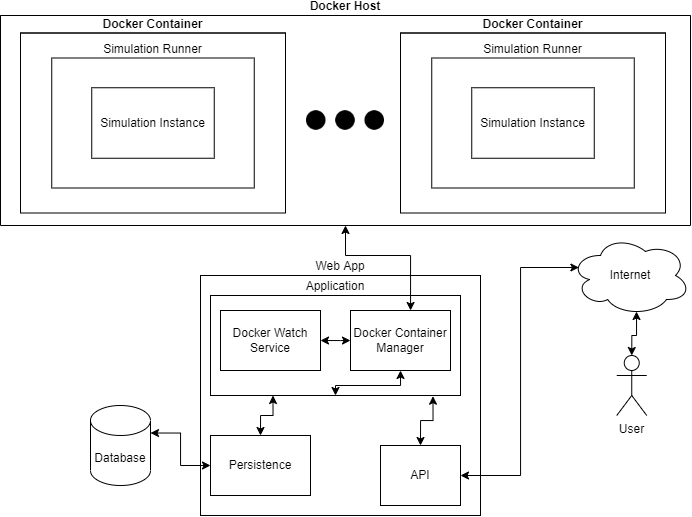
\includegraphics[width=\linewidth]{Component Communication Diagram}
	\caption{Diagram komunikacji między komponentami}
	\label{fig:componentCommunicationDiagram}
	\source{Opracowanie własne.}
\end{figure}

\par Na załączonym powyżej diagramie \ref{fig:componentCommunicationDiagram}, widzimy w jaki sposób komunikują się pomiędzy sobą poszczególne komponenty. Użytkownik wchodzi w interakcję tylko z warstwą \emph{API}, która zajmuje się tylko i wyłącznie obsługą zapytań. Całość logiki biznesowej została oddelegowana do warstwy aplikacji. Ta też warstwa (a konkretnie jej komponent \emph{Docker Container Manger}) jest odpowiedzialna za uruchamianie i zarządzanie kontenerami \emph{\docker{}}a.

\par Za obsługę bazy danych odpowiedzialna jest warstwa \emph{Persistence}. Wszystkie aktywności wymagające przechowania nowych rekordów, aktualizacji lub usunięcia już istniejących są przez nią obsługiwane.

\par \emph{Docker Host} czyli system, na którym jest uruchomiony \emph{\docker{}}. Komunikacja z nim następuje poprzez \emph{Docker Engine API}. Ważnym do zaznaczenia tutaj jest fakt, że może to być albo ten sam \emph{host}, na którym jest uruchomiona nasz aplikacja, ale niekoniecznie musi. Możliwe jest połączanie się z \emph{remote host}em przez internet co prezentuje możliwość na proste poprawienie skalowalności aplikacji w przyszłość. Obecnie jednak założono, że będzie to ten sam \emph{host}, na którym działa aplikacja, co umożliwiło uproszczenie wymiany informacji z kontenerami, która odbywa się poprzez system plików.

\section{Implementacja}

\subsection{Struktura Solucji}

\par W \emph{\dotnet{}} istnieje koncept tak zwanych \emph{solucji}\english{Solutions}. Mają one na celu zgromadzenie w sobie projektów, które razem tworzą rozwiązanie danego zagadnienia. Podejście to pozwala na wyrazisty podział kodu, jak i na wielokrotne jego użycie, zgodne z zasadą \emph{DRY}\footnote{Don't Repeat Yourself}. Odpowiednia zaplanowanie naszego rozwiązania potrafi znacząco przyśpieszyć pracę.

\begin{figure}
	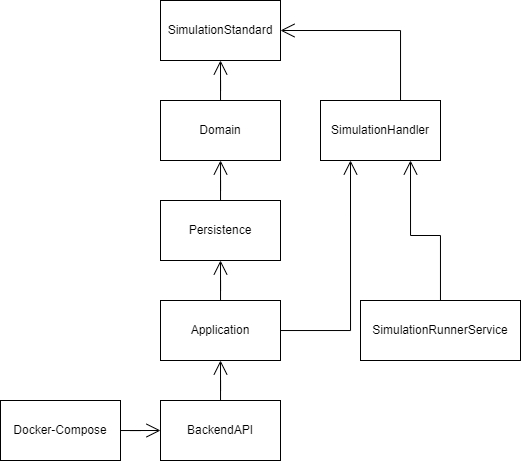
\includegraphics[width=\linewidth]{Solution Structure Diagram}
	\caption{Diagram Struktury Solucji}
	\label{fig:solutionStructureDiagram}
	\source{Opracowanie własne.}
\end{figure}

\par \emph{Docker-Compose} zawiera wszystkie potrzebne informacje do uruchomienia całości rozwiązania, w formie kontenerów \emph{\docker{}}. Umożliwia to uruchomienie aplikacji nie posiadając zainstalowanej platformy \emph{\dotnet{}}, jako iż wszystkie wymagane komponenty zostaną automatycznie pobrane i dodane do odpowiedniego obrazu \emph{\docker{}}.

\par Za punkt wejściowy do naszej aplikacji uznajemy projekt \emph{BackendAPI}. Odpowiada on za uruchomienie i skonfigurowanie wszystkich serwisów. W nim również znajdują się wszystkie kontrolery, logika związana z uwierzytelnianiem użytkownika, jak i pliki konfiguracyjne. \emph{Endpoint}y, które się tutaj znajdują nie posiadają w sobie żadnej logiki biznesowej. Ich zadaniem jest stworzenie odpowiedniego \emph{request}u dla aplikacji, która to dopiero zajmie się jego obsłużeniem.

\par \emph{Application} jest głównym projektem, który spina wszystkie pozostałe. Znajduje się w nim cała logika biznesowa. Odpowiada on za między innymi tworzenie użytkowników i ich autoryzację, zbieranie parametrów i wyników symulacji oraz obsługę pozostałych zapytań, w tym tych związanych z kontenerami (więcej informacji na ten temat znajduje się w sekcjach \ref{sec:dockerContainerManager} i \ref{sec:dockerWatchService}).

\par Odpowiedzialność związana z obsługą symulacji dostarczonych przez użytkowników należy do \emph{SimulationHandler}. Znajduje się tutaj interfejs \texttt{ISimulationHandler} i jego implementację. Klasa ta potrafi tworzyć obiekty \emph{SimulationStandard}, w tym przeprowadzać ich serializację i deserializację. Kolejną istotną cechą jest dynamiczne ładowanie i rozładowanie tak zwanych \emph{Assemblies}, jak i sprawdzanie ich poprawność i zgodności z \emph{SimulationStandard}.

\par Projekty \emph{Persistence} i \emph{Domain} odpowiadają za przechowywanie danych. Działają one w oparciu o \emph{Entity Framework Core}. Pierwszy z nich odpowiada za rozszerzenie tak zwanego \emph{DbContext}\footnote{Specjalna klasa pochodząca z Entity Framework Core definiująca pewien kontekst danych.}, w którym znajdują się deklaracje kolekcji, które będą mapowane do poszczególnych tabel w bazie danych. Znajdują się tutaj również migracje, wspomagające ciągły rozwój aplikacji, poprzez zapewnianie mechanizmu do prostego aktualizowania przechowywanych danych w wypadku zmiany ich struktury. Projekt \emph{Domain} reprezentuje z kolej poszczególne byty na których operuje nasza aplikacja. Są one bezpośrednio mapowane do odpowiednich rekordów. Warstwa ta została zaprojektowana przy pomocy tak zwanego podejścia \emph{Code First}. Oznacza to, że odpowiednie struktury w bazie danych zostały automatycznie wygenerowane na podstawie zdefiniowanych klas.

\par Zadaniem \emph{SimulationRunnerService}u jest uruchomienie wyznaczonej symulacji z odpowiednimi parametrami oraz późniejsze zapisanie wyników. Został on zaimplementowany w oparciu o \texttt{BackgroundService}, który z kolei implementuje \texttt{IHostedService}.\cite{DOTNET_HOSTED_SERVICE} Serwis ten funkcjonuje jako osobny \emph{\docker Image}, który jest uruchamiany jako kontener przez \texttt{IDockerContainerManager}. Całość komunikacji pomiędzy poszczególną instancją i resztą systemu odbywa się przez system plików (więcej informacji na ten temat znajduje się w sekcji \ref{sec:dockerContainerManager}).

\par \emph{SimulationStandard} definiuje strukturę jaką powinna spełniać symulacja przygotowana przez użytkownika, jak i jej obsługiwane typy danych parametrów oraz rezultatów. Temu tematowi poświęcona jest sekcja \ref{sec:simulationStandard}.

\subsection{Zastosowane Wzorce Projektowe}
\label{subsec:zastosowaneWzorceProjektowe}

\par Wzorce projektowe pozwalają programistom w szybszy sposób zaznajomić się z aplikacją, poprzez dodanie kolejnej warstwy aplikacji, jak i rozwiązać problemy, które już kiedyś zostały rozwiązane. Należy jednak pamiętać, że trzeba umiejętnie z nich korzystać i rozważyć zarówno korzyści, jak i potencjalne mankamenty, które mogą z nich wyniknąć. Mając to na uwadze, zdecydowano się użyć następujących \emph{Design Patterns}.

\begin{itemize}
	\item Model View Controller - jeden z najbardziej rozpowszechnionych wzorców projektowych, mówiących o architekturze aplikacji. Wprowadza on prosty podział odpowiedzialności poszczególnych komponentów programu. Został on wybrany ze względu na swoją adekwatność oraz wsparcie ze strony \emph{ASP.NET Core}.
	\item Dependency Injection - wzorzec pozwalający na tworzenie luźno-powiązanych ze sobą komponentów\english{Loosely coupled}. Pozwala on na sprawny rozwój oprogramowania, oraz skłania do wprowadzania dodatkowej abstrakcji. Pozwala on na uzyskanie \emph{Inversion of Control}. Dzięki wykorzystaniu \emph{ASP.NET Core} i istniejącego w nim systemu zarządzania serwisami zastosowanie go nie wiązało się z wykonaniem dodatkowej pracy.
	\item Mediator - wzorzec, według którego lepiej jest gdy istnieje jeden obiekt zarządzający przepływem informacji, niż wiele powiązań pomiędzy mniej znaczącymi elementami.\cite{GOF_DESIGN_PATTERNS} Brak zastosowania tego wzorca, mógłby łatwo doprowadzić do sytuacji, w której kod jest mało czytelny, oraz do wycieków pamięci\english{Memory leak} spowodowanych istnieniem zbędnych referencji pomiędzy obiektami. Aby sprawnie zastosować ten wzorzec, postanowiona skorzystać z pakietu \emph{MediatR}.
	\item Data Transfer Object - wzorzec, mający na celu zamiany obiektu, na jego odpowiednik, zawierający tylko wymagane dane. Pozwala to na przesyłanie mniejszej ilości danych, jak i na upewnienie się, że nie zostaną zwrócone, żadne nieporządne informacje, takie jak na przykład hash hasła użytkownika.
	\item Singleton - jeden z najpopularniejszych wzorców projektowych. Jeżeli jakaś klasa go implementuje, oznacza to, że powinna istnieć tylko jedna jej instancja.\cite{GOF_DESIGN_PATTERNS} W przypadku \emph{ASP.NET Core} istnieje specjalny typ serwisu. Jeżeli z niego skorzystamy, to \emph{framework} podczas korzystania z \emph{Dependency Injection} zapewni istnienie tylko jednego takiego obiektu.
	\item Disposable - wzorzec wykorzystywany w \texttt{C\#} do odpowiedniego zwalniania zasobów zarówno \emph{managed}, jak i \emph{unmanaged}.\cite{DOTNET_DISPOSABLE} Rozwiązuje on problemy takie jak zamknięcie strumieni do plików lub połączenia z bazą danych. Jest on stosowany ze względu na niedeterministyczną naturę \emph{Garbage Collector}a. Aby z niego skorzystać, należy zaimplementować interfejs \texttt{IDisposable}. \emph{ASP.NET Core} potrafi rozpoznać klasy implementujące ten wzorzec i w odpowednim momencie wywołać na nich utylizację\english{Dispose}.
\end{itemize}

\subsection{Simulation Standard}
\label{sec:simulationStandard}

\par Aby poprawnie uruchamiać dostarczony kod, wymagane było stworzenie standardu, który określałby wymagania jak i ograniczenia dotyczące dostarczanych plików. W tym celu powstał \emph{Simulation Standard}. Jest to biblioteka zawierająca interfejsy i podstawowe ich implementacje, obiektów potrzebnych do poprawnej inicjalizacji instancji symulacji.

\par Od użytkownika wymaga się, aby zaimplementował \emph{ISimulationBuilder}, który zwróci symulację. Implementacja ta powinna posiadać przynajmniej jeden bezparametrowy konstruktor.

\begin{figure}[H]
	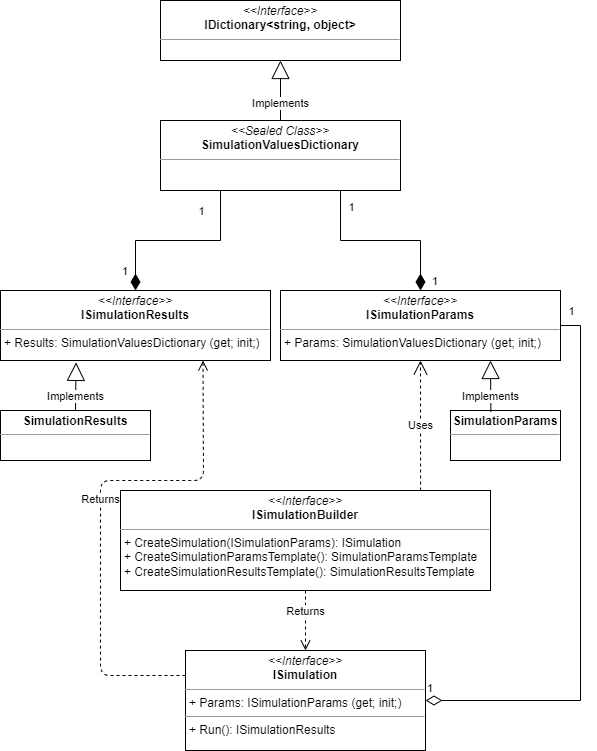
\includegraphics[width=\linewidth]{Simulation Standard Main Diagram}
	\caption{Simulation Standard}
	\label{fig:simulationStandard}
	\source{Opracowanie własne.}
\end{figure}

\par Na załączonym powyżej diagramie (\ref{fig:simulationStandard}) widzimy relację pomiędzy poszczególnymi interfejsami i klasami. Kluczowymi elementami są tutaj \texttt{ISimulationBuilder} oraz \texttt{ISimulation}. Konstruktor ten pozwala, bazując na instancji \texttt{ISimulationParams}, stworzyć symulację, która uruchomiona, zwróci rezultat swojego działania. Zarówno parametry, jak i rezultaty powinny być zgodne z zdefiniowanym szablonem\english{Template}. Powodem tego jest konieczność posiadania dodatkowej informacji potrzebnej do późniejszego poprawnego odtworzenia danych po ich serializacji, jak i w przypadku parsowania zapytania z treścią w formacie \emph{JSON}.

\par \texttt{SimulationValuesDictionary} jest implementacją słownika, która służy do przechowywania wartości parametrów i rezultatów skojarzonych z odpowiednimi nazwami. Odpowiada ona również za kontrolę poprawności danych przechowywanych w niej, dlatego też jest to klasa zapieczętowana\english{Sealed}\footnote{Sealed - klasa, po której nie można dziedziczyć.}. Zostało to dokonane w celu wyraźnego zaznaczenia, że nie powinno się ingerować w jej logikę, ponieważ przysłanianie jej członków może w łatwy sposób prowadzić do niepożądanych rezultatów i błędów aplikacji.

\par Dodatkowo, dla wygody użytkownika, dołączone do biblioteki zostały domyśle implementacje \texttt{SimulationParams} i \texttt{SimulationResults}. Są to proste klasy, które inicjalizują wymagane do swojego funkcjonowania komponenty.

\par Wspomniane wcześniej szablony, służą do zdefiniowania typów danych (oraz ich nazw) jakie będą \emph{input}em i \emph{output}em symulacji. Ich relacje z innymi obiektami można sprawdzić na załączonym poniżej diagramie (\ref{fig:simulationStandardTemplates}). Odpowiedzialnością zbliżone są do \texttt{ISimulationParams} i \texttt{ISimulationResults}, gdzie jedyną różnicą jest to, że nie przechowują wartości ale typy danych. Posiadając wartość parametru w postaci tekstowej, jak i wzorca, który go definiuje jesteśmy wstanie odtworzyć odpowiedni obiekt.

\begin{figure}[H]
	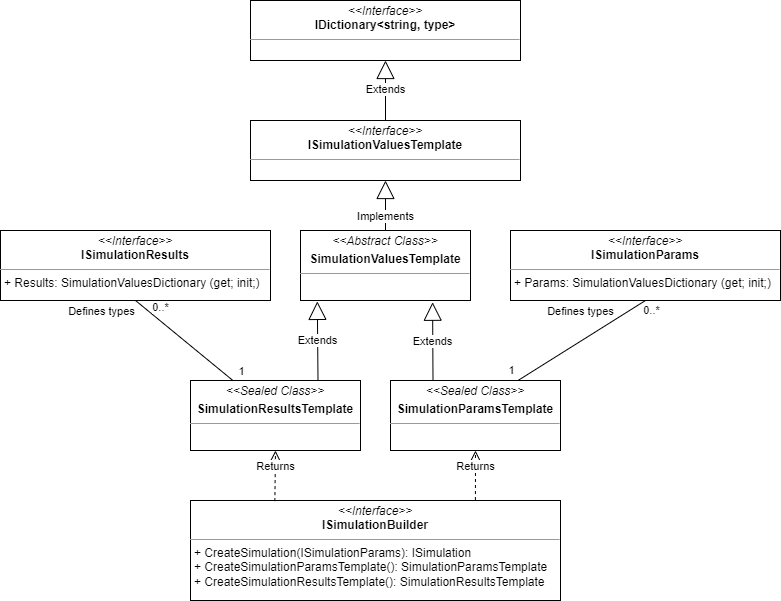
\includegraphics[width=\linewidth]{Simulation Standard Templates Diagram}
	\caption{Simulation Standard Templates}
	\label{fig:simulationStandardTemplates}
	\source{Opracowanie własne.}
\end{figure}

\subsection{Docker Container Manager}
\label{sec:dockerContainerManager}

\par Zarządzanie kontenerami, uruchamianie ich oraz usuwanie i zbieranie rezultatów, zostało oddelegowane do \emph{Docker Container Manager}a. Komponent ten, przy użyciu \texttt{ISimulationHandler}, potrafi przygotować środowisko, w którym zostanie uruchomiony \emph{Simmulation Runner Service}. Wymiana informacji z kontenerem odbywa się poprzez specjalnie przygotowany folder w systemie plików. Menadżer umieszcza tam pliki symulacji, jak i pliki z zserializowanymi danymi, a w późniejszym etapie odbiera stamtąd wyniki.

\par Zastosowano bibliotekę \emph{Docker.Dotnet}, która pozwala na wykonywanie zapytań do \emph{\docker{} Engine API}. Zawiera ona obiekty reprezentujące zarówno parametry zapytań, jak i uzyskane odpowiedzi. Kolejną istotną jej zaletą jest to, że jej implementacja wspiera asynchroniczne mechanizmy platformy \emph{\dotnet{}}.

\par Ponieważ zarówno zapytania do \emph{\docker{} Engine API}, jak i działania na plikach są to operacje, które mogą zająć znaczącą ilość czasu, to istotnym elementem jest obsługa tych działań w sposób asynchroniczny, aby nie blokować wątku. W implementacji skorzystano z mechanizmu \texttt{async/await} platformy \emph{\dotnet{}}. Dzięki czemu system jest w stanie obsłużyć zapytania w krótszym czasie (wątek \emph{request}u nie jest blokowany, a może wykonywać inne działania, zanim będzie konieczne oczekiwanie).

\subsection{Docker Watch Service}
\label{sec:dockerWatchService}

\par Kiedy kontener \emph{\docker{}}a kończy swoje działanie to przechodzi w stan \texttt{exited}. \emph{Docker Watch Service} odpowiada za poszukiwanie takich kontenerów. Serwis ten działa w tle przez cały czas życia aplikacji i w regularnych odstępach czasu sprawdza działające instancje, które zostały zainicjalizowane przez \emph{Docker Container Manager}. Jego działanie prezentuje następujący schemat blokowy.

\begin{figure}[H]
	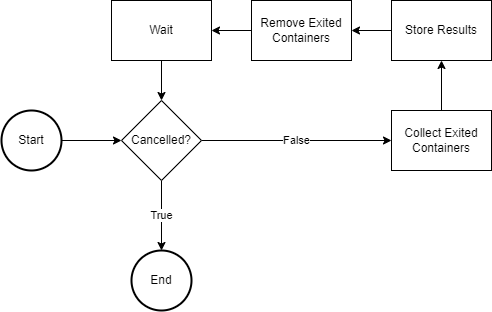
\includegraphics[width=\linewidth]{Docker Watch Service Setps}
	\caption{Docker Watch Service - Schemat Blokowy}
	\source{Opracowanie własne.}
\end{figure}

\par Wszystkie te informacje, można zreasumować w postaci cyklu życia kontenera.

\begin{figure}[H]
	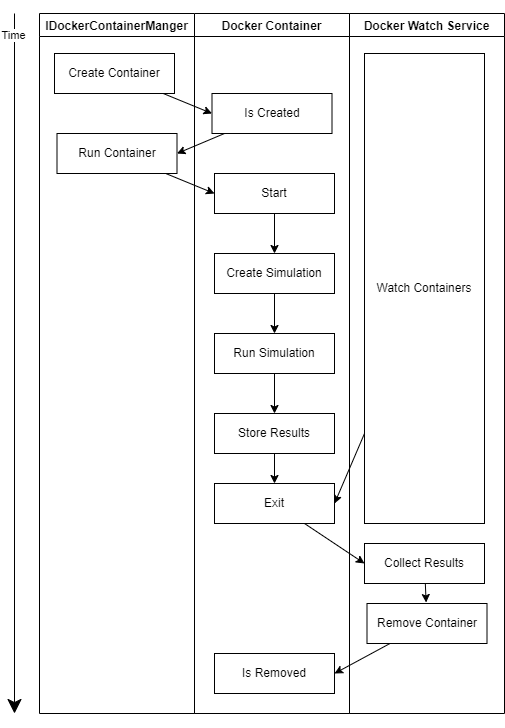
\includegraphics[width=\linewidth, height=0.92\textheight]{Container Lifecycle}
	\caption{Cykl Życia Kontenera}
	\source{Opracowanie własne.}
\end{figure}

\subsection{Schemat Bazy Danych}

\par Zaprojektowanie odpowiedniego schematu bazy danych było jednym z priorytetowych wyzwań podczas tworzenia tej aplikacji. Jej konstrukcja powinna pozwolić na przechowywanie informacji o użytkowniku, plików symulacji, jak i jej parametrów oraz wyników, podzielonych na poszczególne uruchomienia\footnote{Run Attempt}. Dodatkowym wyzwaniem było przechowanie wspomnianych wcześniej danych wejściowych i wyjściowych. Pomogło w tym ograniczenie ich rodzaju w \emph{Simulation Standard}zie (więcej informacji na ten temat można znaleźć w sekcji \ref{sec:simulationStandard}). Ostateczną formą jest zaprezentowany poniżej schemat.

\begin{figure}[H]
	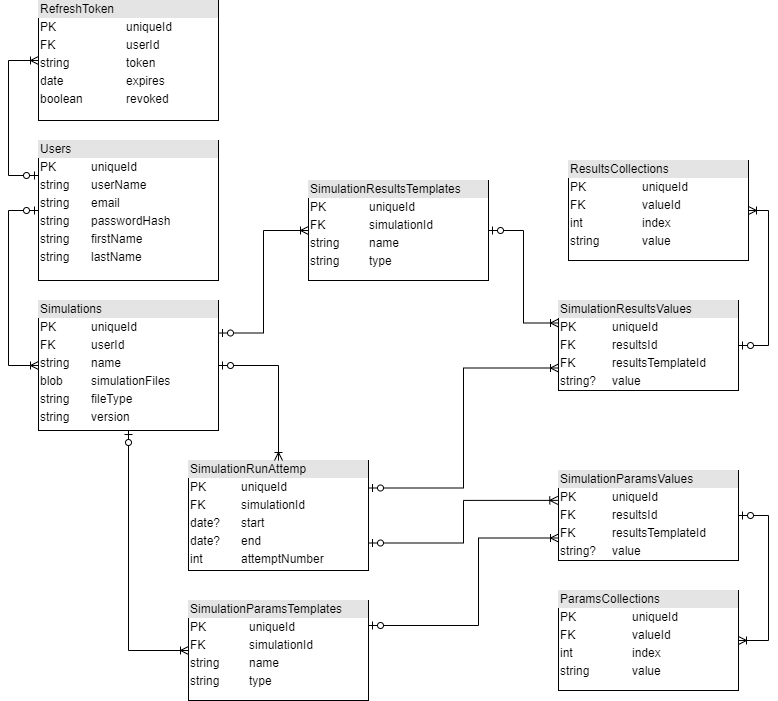
\includegraphics[width=\linewidth]{Database Schema Diagram}
	\caption{Schemat Bazy Danych}
	\source{Opracowanie własne.}
\end{figure}

\par Do jego reprezentacji postanowiono zastosować tak zwaną \emph{Crow's Foot Notation}. Przy procesie tworzenie użyto podejścia \emph{Code First}, co oznacza, że klasy stworzone w \texttt{C\#} są mapowane do odpowiednich tabel. Na schemacie pominięto mniej znaczące elementy (dla przykładu, jako iż klasa \texttt{User} dziedziczy po \texttt{IdentityUser} to jej tabela zawiera informacje potrzebne do pełnego odtworzenia również obiektów tej klasy), aby zachować jego czytelność.

\par Wspomnieć należy tutaj również o ogromnej roli \emph{Entity Framework Core}. Dzięki zapewnionemu przez niego systemowi migracji, możliwe było szybkie dokonywanie zmian w strukturze bazy danych podczas rozwijania aplikacji, bez konieczności usuwania już istniejącej i zaczynania od początku. O ile brak tego mechanizmu spowolniłby proces \emph{development}u, to jego brak nie byłby krytyczny. Tego samego nie można jednak powiedzieć o późniejszym stadium rozwoju. W momencie udostępnienia \emph{software}u użytkownikom, istnienie mechanizmu umożliwiającego wprowadzanie zmian w istniejącej już strukturze danych jest nieocenione.

\section{Wymagania i Konfiguracja}
\label{sec:wymaganiaIKonfiguracja}

\subsection{Wymagania}
\par Aplikację webową, można uruchomić w jednym z dwóch możliwych wariantów (więcej informacji można znaleźć w sekcji \ref{subsec:konfiguracja}). Minimalnym wymaganiem jest system z zainstalowanym \emph{\docker}em w wersji:

\begin{itemize}
	\item \emph{\docker{} Client} - 20.10.11 lub wyższej,
	\item \emph{\docker{} Engine} - 20.10.11 lub wyższej.
\end{itemize}

\par Pozwoli to na uruchomienie programu z użyciem \emph{\docker{} Compose}, który skompiluje wszystkie projekty, uruchomi aplikację w kontenerze\english{Container} oraz utworzy odpowiedni kontener dla bazy danych na bazie oficjalnego obrazu\english{Image} \emph{PostgreSQL}. Podejście to zostało przedstawione w postaci grafiki \ref{fig:wizualizacjaWariantowKonfiguracji} jako wariant pierwszy.

\par Drugim możliwym wariantem jest uruchomienie aplikacji webowej w systemie \emph{host}a. Konieczne jest do tego środowisko \emph{\dotnet{} 6} oraz wspomniany wcześniej \emph{\docker{}}. Konfiguracja ta wymaga samodzielnego uruchomienia kontenera (lub innego środowiska) dla bazy danych \emph{PostgreSQL}. Podejście to zostało przedstawione w postaci grafiki \ref{fig:wizualizacjaWariantowKonfiguracji} jako wariant drugi. Baza danych nie została tutaj zaprezentowana, ponieważ nie istnieje wymaganie, aby była ona obecna w systemie \emph{host}a. Możliwym jest posłużenie się zdalną bazą danych poprzez zapewnienie odpowiedniego \emph{Connection String}.

\begin{figure}[H]
	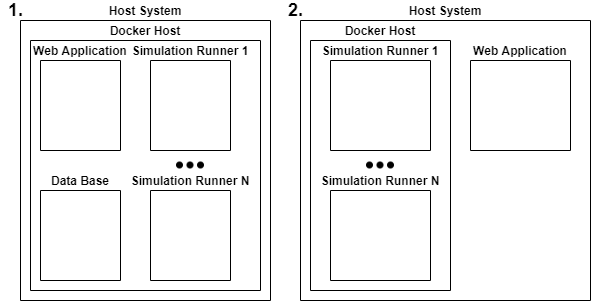
\includegraphics[width=\linewidth]{Configuration Variants Diagram}
	\caption{Wizualizacja Wariantów Konfiguracji}
	\label{fig:wizualizacjaWariantowKonfiguracji}
	\source{Opracowanie własne.}
\end{figure}

\par Przed uruchomieniem wymagane jest również stworzenie odpowiedniego obrazu \emph{\docker{}}a na bazie pliku \emph{Dockerfile} znajdującego się w projekcie \emph{SimulationRunnerService}. Można tego dokonać przy użyciu komendy:

\begin{lstlisting}
	docker build -t simulationrunnerservice -f .\SimulationRunnerService\Dockerfile .
\end{lstlisting}

\subsection{Konfiguracja}
\label{subsec:konfiguracja}

\par Do odpowiedniego skonfigurowania aplikacji wykorzystuje się pliki \emph{launchSettings.json} i \emph{appsettings.json}. Znajdują się one w projekcie \emph{BackendAPI} i posiadają wiele możliwych wariantów (na przykład istnieje \emph{appsettings.json} i \emph{appsettings.Development.json}). Odpowiedni plik konfiguracyjny jest wybierany na podstawie ustawienia odpowiedniej zmiennej środowiskowej (\texttt{ASPNETCORE\_ENVIRONMENT}) lub parametru przekazywanego podczas uruchamiania aplikacji przy użyciu \emph{\dotnet{}} \emph{CLI}\footnote{Command Line Interface}.

\newcommand{\onlyConfiguration}[1]{(dotyczy tylko konfiguracji numer #1 z grafiki \ref{fig:wizualizacjaWariantowKonfiguracji})}

\par Dla plików \emph{appsettings.json}, parametry jakie należy dostarczyć to:
\begin{itemize}
	\item \texttt{TokenKey} - klucz dla tokenów,
	\item \texttt{JWT}:
	\begin{itemize}
		\item \texttt{Audience} - odbiorcy tokenu,
		\item \texttt{Issuer} - nadawca tokenu,
	\end{itemize}
	\item \texttt{SimulationRunnerServiceDockerImage} - ID lub nazwa obrazu \emph{\docker{}},
	\item \texttt{DockerHostContainersPath} - ścieżka dostępu do folderu przeznaczonego na dane kontenerów \onlyConfiguration{1},
	\item \texttt{ConnectionStrings}:
	\begin{itemize}
		\item \texttt{PostgreSQL} - \emph{Connection String} definiujący połączenie z bazą danych \onlyConfiguration{2},
		\item \texttt{PostgreSQLDocker} - służy dokładnie temu samemu celowi co \texttt{PostgreSQL}. Aby usprawnić proces rozwijania aplikacji, jak i ułatwić jej testownie, utworzone dwie zmienne \onlyConfiguration{1}.
	\end{itemize}
\end{itemize}

\par Dodatkowo należy dostarczyć następujące dane w postaci \emph{\dotnet{} Secret}:
\begin{itemize}
	\item \texttt{Postgres}:
	\begin{itemize}
		\item \texttt{user} - nazwa użytkownika bazy danych,
		\item \texttt{password} - hasło użytkownika bazy danych,
	\end{itemize}
	\item \texttt{Kestrel:Certificates:Development:Password} - hasło dla certyfikatu. Zmienna ta może się różnić w zależności od środowiska i certyfikatu jaki jest wykorzystywany. Dla testów użyto \emph{Self-Signed Certificate} wygenerowanego przy użyciu narzędzia \emph{dotnet dev-certs}.\cite{DOTNET_SELFSIGNED_CERTIFICATE}
\end{itemize}

Aby tego dokonać, należy skorzystać z \emph{Secret Manager}a.\cite{DOTNET_SECRET_MANAGER}

\section{Endpoints}

\par Powstała aplikacja działa jako \emph{API}, co za tym idzie posiada tak zwane \emph{Endpoint}y, czyli adresy \emph{URL}, do których należy się odwołać aby wywołać pożądane działanie lub uzyskać zamierzone dane. Udostępnione zostały \emph{endpoint}y pozwalające na:
\begin{itemize}
	\item zarejestrowanie użytkownika,
	\item zalogowanie użytkownika,
	\item uzyskanie informacji o użytkowniku,
	\item wgranie symulacji,
	\item uzyskanie informacji o wgranych wcześniej symulacjach,
	\item uruchomienie symulacji, korzystając z podanych parametrów,
	\item uzyskanie wszystkich wyników symulacji,
	\item uzyskanie jednego, wybranego wyniku symulacji.
\end{itemize}

\par \emph{Endpoint}y zwracają zarówno odpowiedni kod statusu \texttt{HTTP}\english{HTTP Status Code}, ale również odpowiedzi w formacie \emph{JSON}. Z niektórych \emph{endpoint}ów można korzystać bez odpowiedniego upoważnienia\english{Authorization}, jednak większość z nich wymaga posiadania konta użytkownika. Aby poprawnie przejść przez proces uwierzytelniania, musimy wraz z zapytaniem przesłać odpowiedni token. Token ten jest ważny przez z góry określoną ilość czasu i aby go odświeżyć, należy wysłać zapytanie do \emph{/api/User}.

\par Dzięki skorzystaniu z technologii \emph{Swagger} została wygenerowana również specjalna strona internetowa, przy użyciu której można sprawdzić wszystkie dostępne \emph{endpoint}y, wraz z przykładami ich użycia oraz przykładowymi odpowiedziami ze strony serwera (więcej informacji na ten temat można znaleźć w sekcji \ref{subsec:swagger}). Strona ta jest dostępna pod adresem: \emph{https://\texttt{ADRES SERWERA}/swagger/index.html}.

\begin{figure}[H]
	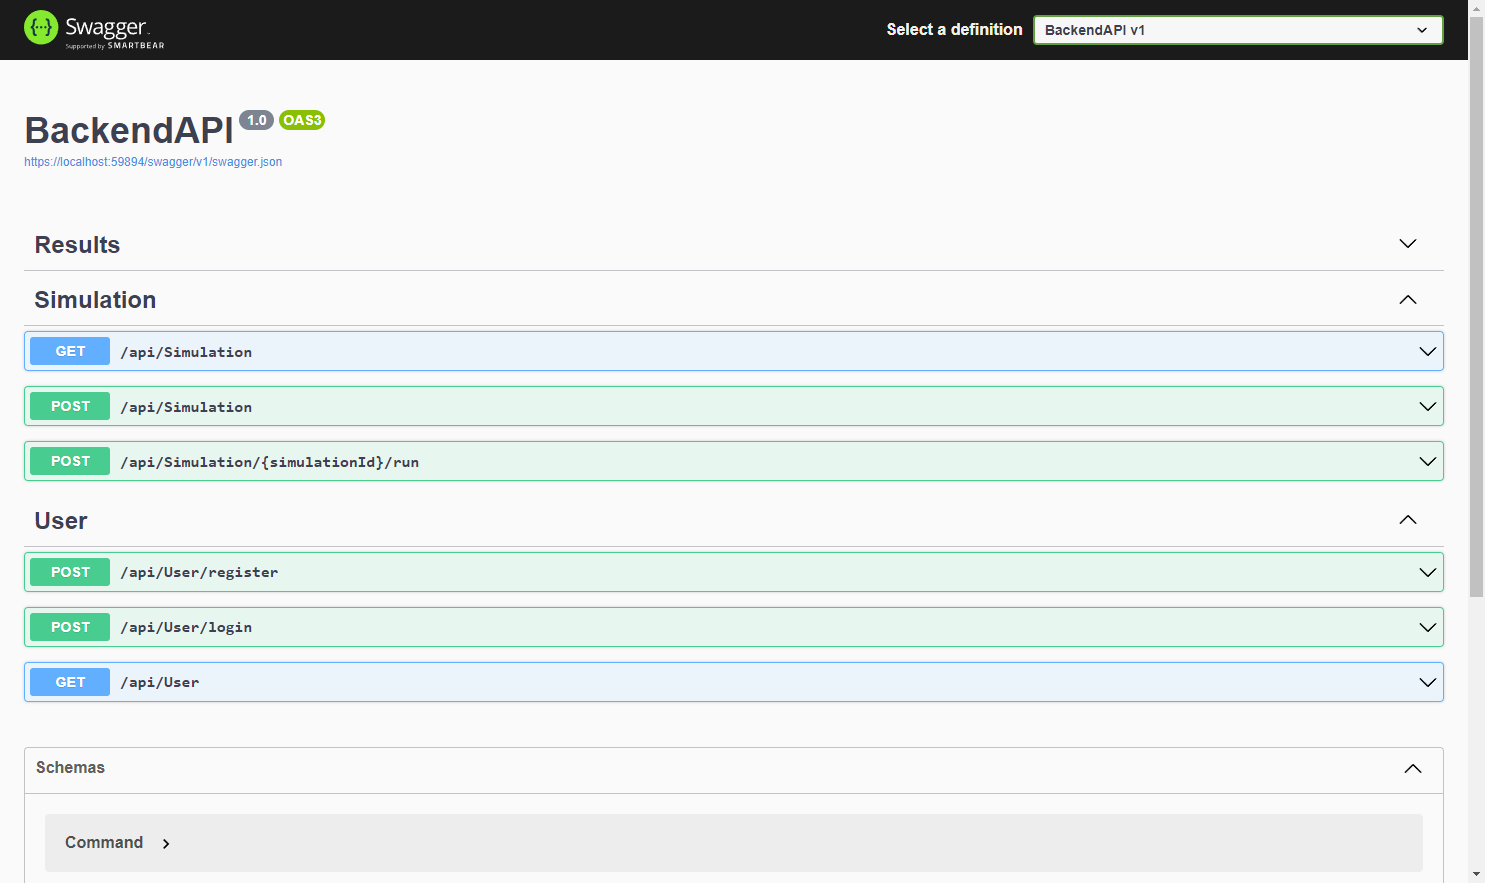
\includegraphics[width=\linewidth]{Swagger Presentation}
	\caption{Prezentacja Swaggera}
	\source{Opracowanie własne.}
\end{figure}

\par Wartym dodatkowej uwagi jest \emph{endpoint}: \texttt{POST} \emph{/api/Simulation}, ze względu na to, iż weryfikuje on zawartość przesłanego pliku i sprawdza jego zgodność ze standardem. Wykonuje on testy na to, czy zostały zaimplementowane \texttt{ISimulation} oraz \texttt{ISimulationBuilder}, czy istnieje bezparametrowy konstruktor oraz tworzy odpowiednie szablony dla parametrów i rezultatów symulacji. Co za tym wszystkim idzie, wczytuje on przesłany plik i uruchamia kod pochodzący z niego. \emph{Endpoint} ten niestety nie deleguje tego zadania do specjalnego kontenera, ale wykonuje wszystkie działania samodzielnie. Powoduje to istnienie potencjalnej luki bezpieczeństwa. W przypadku chęci udostępnienia tej aplikacji do szerszej publiki, działanie tego \emph{endpoint}u powinno zostać zmienione i również korzystać z konteneryzacji celem bezpiecznego uruchamiania kodu \emph{3\textsuperscript{rd}-party}.

\par Aby przesłana symulacja została poprawnie obsłużona przez system, powinna ona implementować \texttt{ISimulationBuilder} oraz \texttt{ISimulation} z biblioteki \emph{Simulation Standard} (więcej informacji na ten temat znajduje się w sekcji \ref{sec:simulationStandard}). Dodatkowo \emph{builder} powinien posiadać bezparametrowy konstruktor. Całość powinna zostać skompilowana do pojedynczego pliku \texttt{.DLL}. Jest to obecne ograniczenie systemu, które może zostać rozwiązane w przyszłości (więcej informacji na ten temat znajduje się w sekcji \ref{subsec:obslugaSymulacjiSkladajacychSieZWieluAssembly}).

\section{Obsługa błędów}

\par Aplikacje komputerowe powinny być tworzone z myślą o obsłudze potencjalnych błędów. Przez błędy mamy tutaj na myśli zarówno błędy po stronie użytkownika, jak i błędy, za które odpowiedzialny jest serwer. Taki też podział zastosowano w tym projekcie. Aby obsłużyć w odpowiedni sposób wszystkie sytuacje wyjątkowe, wykorzystano tutaj mechanizm wyjątków\english{Exceptions}.

\par Błędy użytkownika można podzielić na dwa rodzaje:
\begin{itemize}
	\item związane z odpowiednimi upoważnieniami,
	\item związane z niepoprawnymi danymi lub niepoprawnym ich formatem.
\end{itemize}
Pierwsze z nich są obsługiwane przez mechanizm upoważniania z \emph{ASP.NET Core}, który dzięki dodaniu odpowiedniej polityki\english{Policy}, weryfikuje czy dany użytkownik istnieje, jak i to czy jest właścicielem danej symulacji. W przypadku błędu, system zwróci odpowiedni kod, czyli \emph{Unauthorized} lub \emph{Forbidden} w zależności od etapu na jakim wystąpiło niepowodzenie. Drugi rodzaj jest natomiast obsługiwany na etapie dalszej walidacji i wykonywania danego zapytania. W przypadku błędu zwróci on odpowiedni kod (\emph{Bad Request}), jak i informację na temat błędu. Dla przykładu, gdy odpowiedni \emph{Run Attempt} nie zostanie odnaleziony, odpowiedzią od serwera będzie \texttt{400 Bad Request} i następujący obiekt \emph{JSON}.

\begin{lstlisting}
{
	"errors": {
		"RunAttempt": "Not found."
	}
}
\end{lstlisting}

\par Jeżeli w trakcie obsługi zapytania wystąpi inny błąd, to zostanie do użytkownika zwrócona odpowiednia informacja oraz \texttt{500 Internal Server Error}. Odpowiedni \emph{stack-trace} zostanie wyświetlony w konsoli i jeżeli będzie istnieć taka możliwość, to aplikacja podejmie próbę kontynuacji swojego działania. Dotyczy to się również innych błędów mogących wystąpić bez ingerencji użytkownika, na przykład w trakcie działania \emph{Docker Watch Service}.

\section{Prezentacja działania aplikacji}

\par Jako iż formą aplikacji jest \emph{API}, to jedyną możliwą formą prezentacji jej działania jest wykonanie odpowiednich zapytań i prezentacja rezultatów. W procesie rozwijania, jak i testowania projektu skorzystano z aplikacji \emph{Postman}. Umożliwił on proste tworzenie zapytań, uzyskiwanie ich rezultatów, jak i uruchamianie testów. Poniżej widzimy przykładowe, prawidłowe zapytanie i uzyskaną odpowiedź.

\begin{figure}[H]
	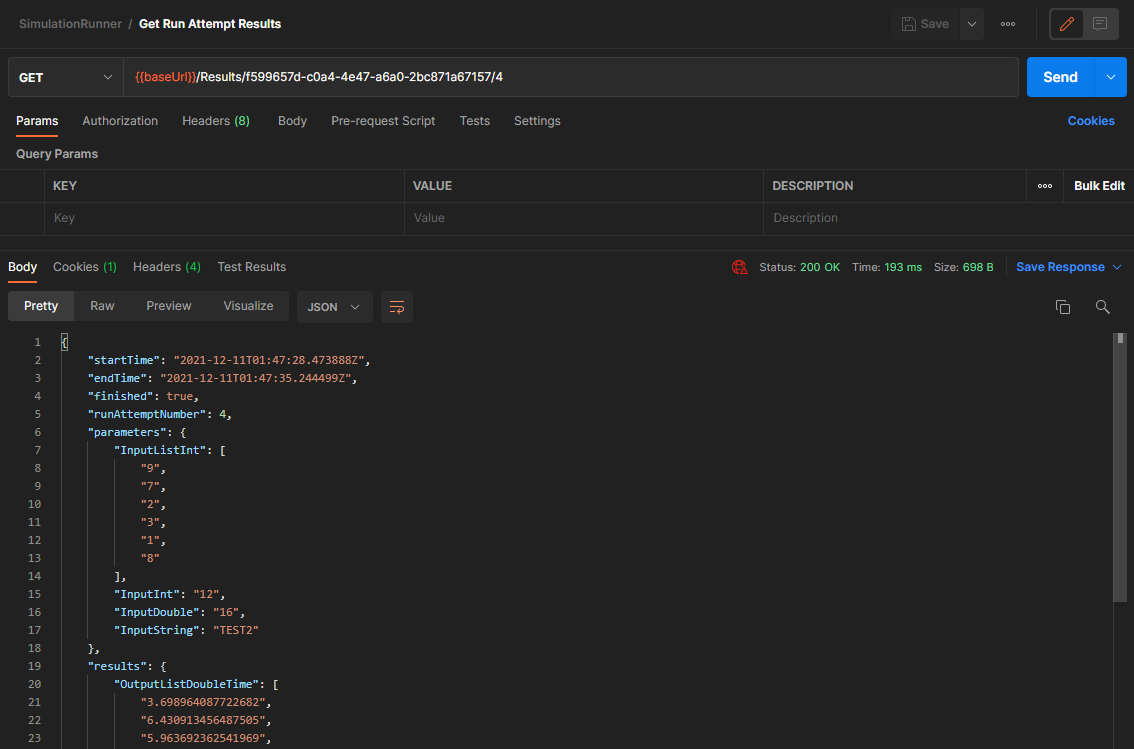
\includegraphics[width=\linewidth]{Postman Simulation Results Correct Request}
	\caption{Postman - Rezultat prawidłowego zapytania}
	\source{Opracowanie własne.}
\end{figure}

\par Prawidłowe działanie aplikacji można również zaobserwować instalując \emph{Docker Desktop} (lub korzystając z innych narzędzi \emph{\docker{}}a na przykład w terminalu). Poniżej przedstawiono dwa zrzuty ekranu pokazujące uruchomione kontenery, a następnie ich usunięcie.

\begin{figure}[H]
	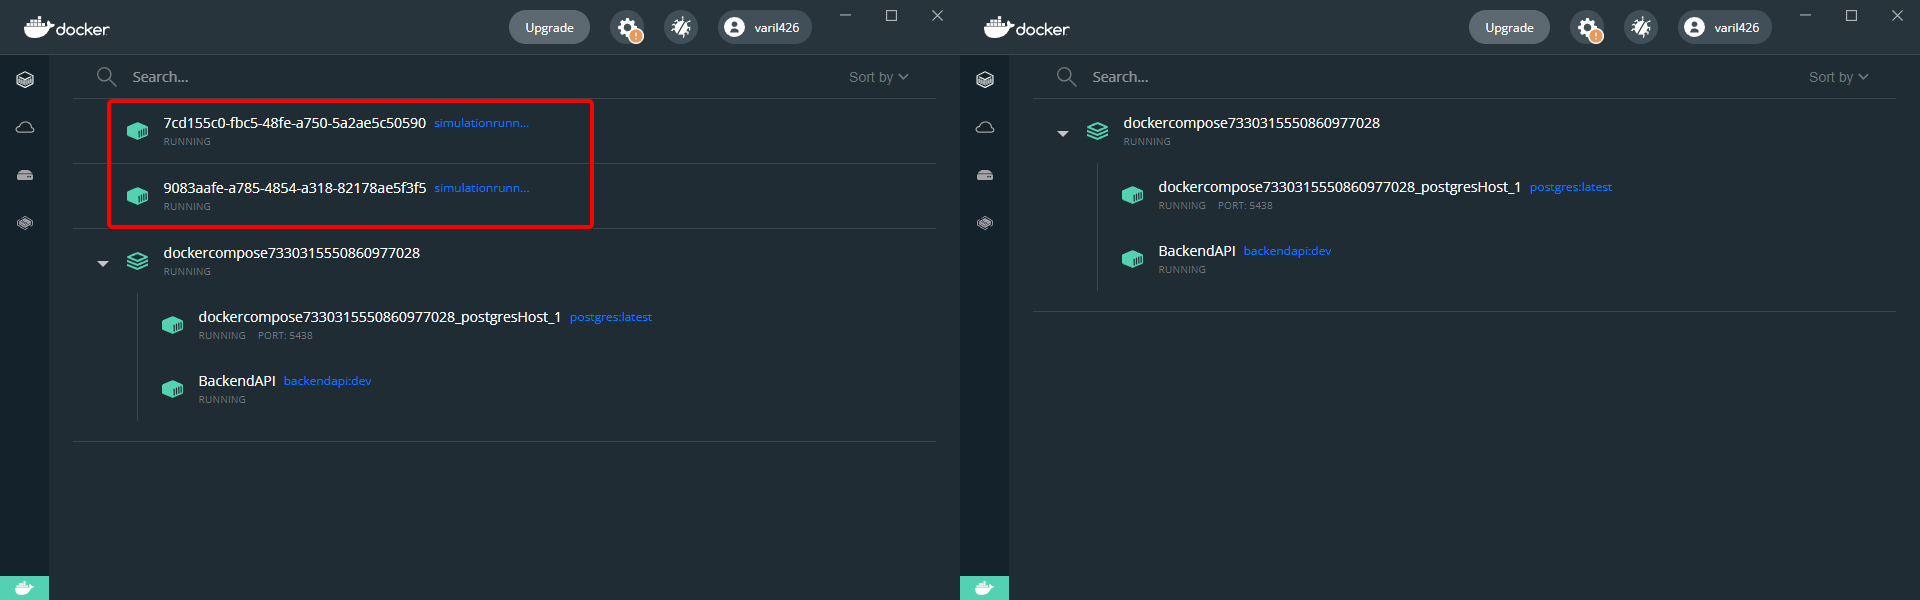
\includegraphics[width=\linewidth]{Docker - Running SimulationRunnerService}
	\caption{Docker Desktop - Uruchomione, a następnie usunięte kontenery}
	\source{Opracowanie własne.}
\end{figure}

\section{Testy}

\subsection{Testy funkcjonalności związanej z obsługą użytkownika}

\par W ramach testowania funkcjonalności związanej z obsługą użytkownika wykonano testy polegające między innymi na:
\begin{itemize}
	\item stworzeniu nowego konta:
	\begin{itemize}
		\item z poprawnymi danymi,
		\item z niepoprawnymi lub brakującymi danymi,
	\end{itemize}
	\item logowaniu się,
	\item próbie uzyskanie dostępu do danych bez odpowiednich upoważnień,
	\item wgraniu różnych pliku z symulacjami do systemu, jak i plików zawierających niepoprawne dane.
\end{itemize}

Wszystkie testy zakończyły się powodzeniem. Uzyskano oczekiwane rezultaty w formie odpowiedzi ze strony serwera oraz odpowiedniego kodu \emph{HTTP}.

\subsection{Mock Simulation}

\par Aby przetestować działanie aplikacji, została stworzona specjalna symulacja. Miała ona za zadanie wczytanie danych różnych typów, odczekanie pewnej ilości czasu aby zasymulować działanie realnej symulacji oraz stworzenie rezultatów swojego działania bazując na danych wejściowych. Z symulacji tej korzystano w trakcie rozwoju aplikacji.

\subsection{Rabbit Island Simulation}
\label{subsec:rabbitIslandSimulation}

\par W ramach przedmiotu ``Studio Projektowe 2`` pod opieką dr. inż. Jacka Piwowarczyka i przy współpracy z Panią M. Pinior oraz Panem S. Lepianką, powstała symulacja wyspy królików. Jej założeniem jest symulowanie ekosystemu, w którym żyją króliki oraz wilki. Zadaniem królików jest poszukiwanie pożywienia, występującego w formie owoców, natomiast celem wilków jest polowania na wspomniane wcześniej ssaki zającowate. Oba gatunki są dodatkowo zdolne do prokreacji, gdzie generowanie potomstwa może następować według jednego z dwóch dostępnych algorytmów. Symulacja ta posiada wiele opcji konfiguracji, między innymi to czy zwierzęta mają umierać śmiercią naturalną, ile owoców powinno pojawić się każdego dnia oraz jaka powinna być wielkość każdej z populacji na starcie. Symulację tą postanowiono wykorzystać jako obiekt testowy, z powodu iż jej logika jest bardziej zaawansowana, jak i tego, że jej implementacja wykorzystuje wielowątkowe możliwości platformy \emph{\dotnet{}}.

\par Symulacja została uruchomiona w kilku konfiguracjach testowych, w celu sprawdzenia poprawności jej działania oraz z normalnymi parametrami. Wspomniane wcześniej konfiguracje testowe, polegały na ustawieniu skrajny wartości parametrów. Przykładem może tutaj być uruchomienie symulacji z zerową populacją królików, co spowodowało wyginięcie wilków z głodu. Wszystkie obiegi testowe spełniały oczekiwania i ich rezultaty pokrywały się z wynikami otrzymanymi, gdy symulację uruchamiano nie korzystając z \emph{Simulation Runner}a. Więcej informacji na ten temat znajduje się w dodatku \ref{app:wynikiSymulacjiWyspyKrolikow}.
\chapter{Podsumowanie}
\label{cha:podsumowanie}

% itd.
\appendix
\chapter{Wyniki Symulacji Wyspy Królików}
\label{app:wynikiSymulacjiWyspyKrolikow}

\par W ramach procesu testowania aplikacji postanowiono wykorzystać symulację "Wyspy Królików" (więcej informacji można znaleźć w sekcji \ref{subsec:rabbitIslandSimulation}). Symulacja ta zawiera następujące parametry wejściowe:

\begin{center}
	\texttt{
		\begin{tabular}{|c | c | c |}
			\hline
			Nazwa Parametru & Typ & Przyjęta Wartość \\
			\hline
			\hline
			RabbitsInitialPopulation & long & Zmienna w zależności od testu \\
			\hline
			RabbitsMinChildren & long & 0 \\
			\hline
			RabbitsMaxChildren & long & 6 \\
			\hline
			RabbitsPregnancyDuration & long & 2 \\
			\hline
			RabbitsLifeExpectancy & long & 6 \\
			\hline
			WolvesInitialPopulation & long & Zmienna w zależności od testu \\
			\hline
			WolvesMinChildren & long & 0 \\
			\hline
			WolvesMaxChildren & long & 6 \\
			\hline
			WolvesPregnancyDuration & long & 4 \\
			\hline
			WolvesLifeExpectancy & long & 14 \\
			\hline
			TimeRate & long & 3600 \\
			\hline
			DeathFromOldAge & boolean & true \\
			\hline
			MaxCreatures & long & 500 \\
			\hline
			FruitsPerDay & long & 60 \\
			\hline
			MapSize & long & 500 \\
			\hline
			MutationChance & double & 0 \\
			\hline
			MutationImpact & double & 0 \\
			\hline
			OffspringGenerationMethod & long & 0 \\
			\hline
			Timeout & long & 600 \\
			\hline
		\end{tabular}
	}
\end{center}

Wartymi szczególnej uwagi są tutaj:
\begin{itemize}
	\item \texttt{MaxCreatures} - określa maksymalną ilość stworzeń symulowanych w tym samym czasie.
	\item \texttt{TimeRate} - parametr ten decyduje o ile razy szybciej będą działy się wydarzenia w symulacji niż w rzeczywistości. W naszym przypadku przyjmuje on wartość \emph{3600}, co oznacza, że \emph{1} sekunda czasu rzeczywistego to \emph{1} godzina czasu symulowanego.
	\item \texttt{DeathFromOldAge} - jeżeli ustawiony na wartość \texttt{true}, to wartości \texttt{RabbitsLifeExpectancy} i \texttt{WolvesLifeExpectancy} są brane pod uwagę i kreatury umierają nie tylko w wyniku obrażeń, ale i ze starości.
	\item \texttt{Timeout} - określa po jakim czasie (wyrażonym w sekundach czasu rzeczywistego) symulacja ma zostać przerwana.
\end{itemize}

Natomiast za pomocą \texttt{RabbitsInitialPopulation} i \texttt{WolvesInitialPopulation} będziemy sterować początkowymi populacjami ssaków na wyspie. Symulacja kończy się w momencie wymarcia wszystkich kreatur lub przekroczeniu czasu \texttt{Timeout}.

\subsection{Test 1: Zerowa populacja królików}

\par W przypadku pierwszego testu, postanowiona sprawdzić czy założenia symulacji pokryją się z otrzymanymi wynikami. Przy zerowej populacji królików, wszystkie wilki powinny po pewnym czasie wymrzeć z głodu. Sukces tego testu możemy zaobserwować na grafie \ref{fig:rabbitIslandTest1Diagram1}, który powstał na bazie otrzymanych wyników. Początkową populację ustawiono na \emph{14}.

\begin{figure}
	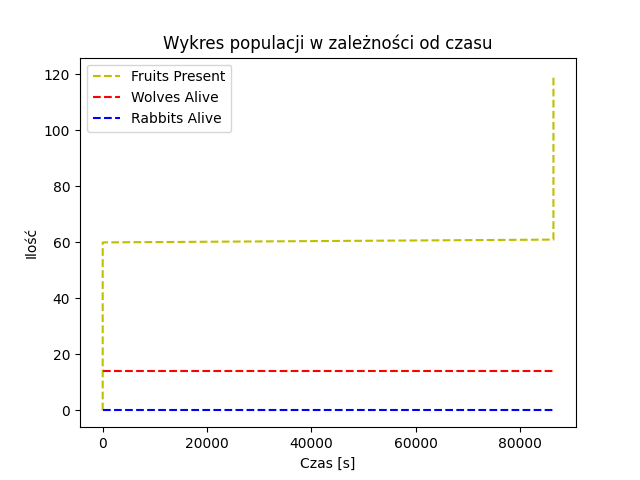
\includegraphics{RabbitIsland - Test 1}
	\label{fig:rabbitIslandTest1Diagram1}
	\caption{Wyspa Królików - Test 1 Diagram}
	\source{Opracowanie własne.}
\end{figure}

\subsection{Test 2: Zerowa populacja wilków}

\par Drugi test sprawdza sytuację analogiczną do pierwszej, tym razem jednak z królikami w roli głównej. Ilość stworzeń na start ustawiono na \emph{14}. Przewidywane są dwa poprawne rezultaty:
\begin{itemize}
	\item Populacja królików urośnie do takiego stopnia, że przychód nowych owoców nie będzie w staniej jej utrzymać. Następnie zacznie się nagłe wymieranie, spowodowane niedostatkiem pokarmu.
	\item Zostanie osiągnięty pewien poziom, na którym populacja królików ustabilizuje się.
\end{itemize}

\begin{figure}
	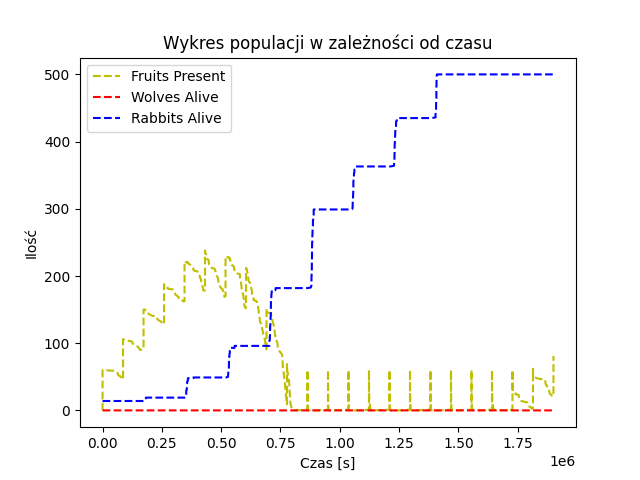
\includegraphics{RabbitIsland - Test 2}
	\label{fig:rabbitIslandTest2Diagram1}
	\caption{Wyspa Królików - Test 2 Diagram}
	\source{Opracowanie własne.}
\end{figure}

\par Na bazie otrzymanego wyniku (grafika \ref{fig:rabbitIslandTest2Diagram1}), możemy stwierdzić, że spełnił się drugi z przewidywanych scenariuszy, jednak nie ze względu na naturalną stabilizację, ale twardy limit stworzeń, ustawiony przez jeden z parametrów. Okresem wzbudzającym zainteresowanie, jest pierwsze kilka dni, gdzie widzimy, jak gromadzi się nadmiar owoców. Ilość owoców osiągnęła swoje globalne maksimum na początku piątego dnia. Rezultaty tego dostatku, możemy zaobserwować w następnych dniach, gdzie występują największe przyrosty populacji królików (koreluje to z ustawionym czasem trwania ciąży - \emph{2 dni}).

\subsection{Test 3: Mieszanie wilków z królikami}

\par Ostatni z wykonanych testów miał za zadanie sprawdzić interakcję pomiędzy dwoma typami stworzeń. Początkowe populacje zostały ustawione na \emph{14} wilków i \emph{24} króliki. Wszystkie pozostałe parametry pozostały bez zmian.

\begin{figure}
	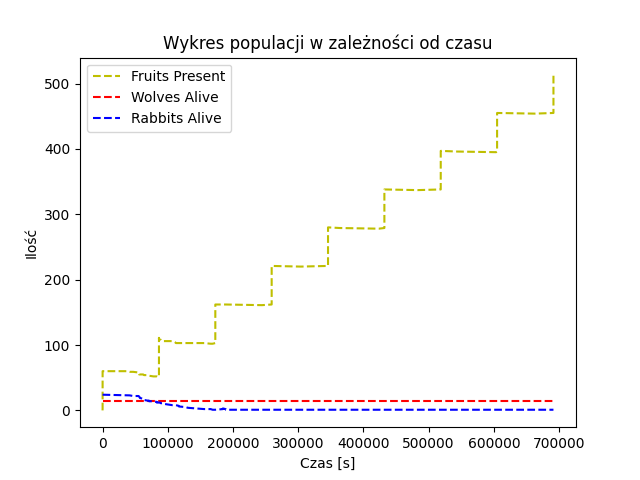
\includegraphics{RabbitIsland - Test 3 1}
	\label{fig:rabbitIslandTest3Diagram1}
	\caption{Wyspa Królików - Test 3 Diagram 1}
	\source{Opracowanie własne.}
\end{figure}

\begin{figure}
	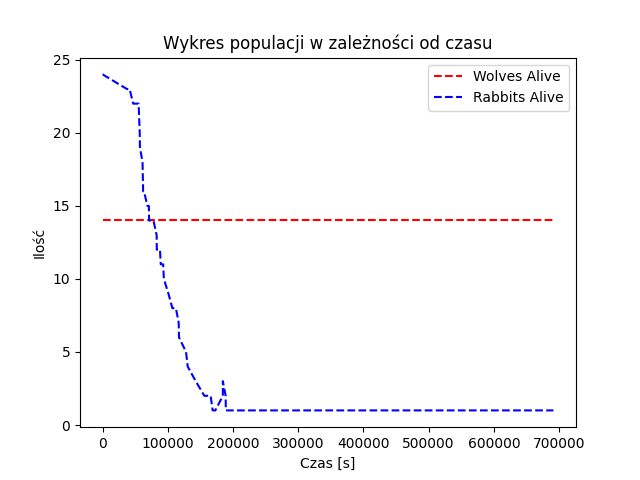
\includegraphics{RabbitIsland - Test 3 2}
	\label{fig:rabbitIslandTest3Diagram2}
	\caption{Wyspa Królików - Test 3 Diagram 2}
	\source{Opracowanie własne.}
\end{figure}

\par Z otrzymanych rezultatów (grafiki \ref{fig:rabbitIslandTest3Diagram1} i \ref{fig:rabbitIslandTest3Diagram2}) możemy wywnioskować, że takie dobranie populacji było nietrafione. Ze względu na stosunkowo nieduży rozmiar mapy, jak i dużą ilość drapieżników populacja królików szybko zmalała do pojedynczego przedstawiciela tego gatunku. Co z kolei spowodowało iż owoce zaczęły się gromadzić, jak i doprowadziło finalnie populację wilków do wymarcia z powodu głodu.


% \include{dodatekB}
% itd.

\printbibliography

\end{document}
